%!TEX root = ../../fourthYearReport.tex

\paragraph{Work package 5 progress}

The activities in WP5 are divided into four tasks corresponding to the four years project duration. As a result, during the fourth year CoDyCo results concentrate on T5.4. The main result consist in the implementation of the validation scenario consisting of the balancing with the help of a caregiver. The main scientific contribution is described here \cite{latella2016whole}.

\subparagraph{Scenario 4: learning how to stand up with the help of a human caregiver (T5.4)}

The main contributions to T5.4 have been presented in ``Validation scenario 4: learning how to stand up with the help of a human caregiver'' which discusses the technical implementation of the fourth year validation scenario (see \url{https://github.com/robotology-playground/codyco-deliverables/tree/master/D5.4/pdf}). The software developed for the scenario implementation is released with an open-source license and distributed through github (\url{https://github.com/robotology/codyco}).


\textbf{CoM Dynamic Manipulability for the iCub in a Sitting Configuration}


In this calculations, it is assumed that the robot is in a sitting
configuration with joint angles mentioned in Table \ref{jointangles}.
Shoulder pitch angle ($\alpha$) and elbow angle ($\beta$) are the two
variables which are used to maximize the CoM dynamic manipulability in a
desired direction.  The desired direction of the CoM movement in the beginning
of the motion is horizontal.  The maximum joint torques are assumed to be
$40$N.m. for the legs and $20$N.m. for the arms.
%
\begin{table} 
  \centering
  \caption{iCub joint angles in a sitting configuration.  Angles are in
    degrees.}
  \begin{tabular}{|c|c||c|c||c|c|}
    \hline hip pitch   & $91$   & shoulder roll & $12$ & torso pitch & $18$ \\
    \hline hip roll    & $12$   & shoulder yaw  & $80$ & torso roll  & $0$   \\
    \hline hip yaw     & $0$    & wrist pronos  & $0$  & torso yaw   & $0$   \\
    \hline knee        & $-104$ & wrist pitch   & $0$  & neck pitch  & $0$ \\
    \hline ankle pitch & $-12$  & wrist yaw     & $0$  & neck roll   & $0$ \\
    \hline ankle roll  & $0$    &               &      & neck yaw    & $0.5$ \\
    \hline
  \end{tabular}
  \label{jointangles}
\end{table}
%
\begin{figure}
  \centering
  \includegraphics[scale=0.29]{3Dfigure.pdf}
  \caption{CoM dynamic manipulability with respect to arm configuration.}
  \label{3Dfig}
\end{figure}
%

The CoM dynamic manipulability for different arm configurations
(i.e. different $\alpha$ and $\beta$) is shown in Figure \ref{3Dfig}.  The
maximum manipulability is at $\alpha = -33^\circ$ and $\beta = 30^\circ$.
Figures \ref{2Dfig_shoulder} and \ref{2Dfig_elbow} show CoM manipulability
with respect to the shoulder angle and the elbow angle, respectively.  Figure
\ref{icub_optimum} show the iCub's configuration when the arms angles are in
their optimum values.
%
\begin{figure}
  \centering \includegraphics[scale=0.4]{2DfigureShoulder.pdf}
  \caption{CoM dynamic manipulability with respect to shoulder pitch angle.}
  \label{2Dfig_shoulder}
\end{figure}
%
\begin{figure}
  \centering
  \includegraphics[scale=0.4]{2DfigureElbow.pdf}
  \caption{CoM dynamic manipulability with respect to elbow angle.}
  \label{2Dfig_elbow}
\end{figure}
%
\begin{figure}
  \centering 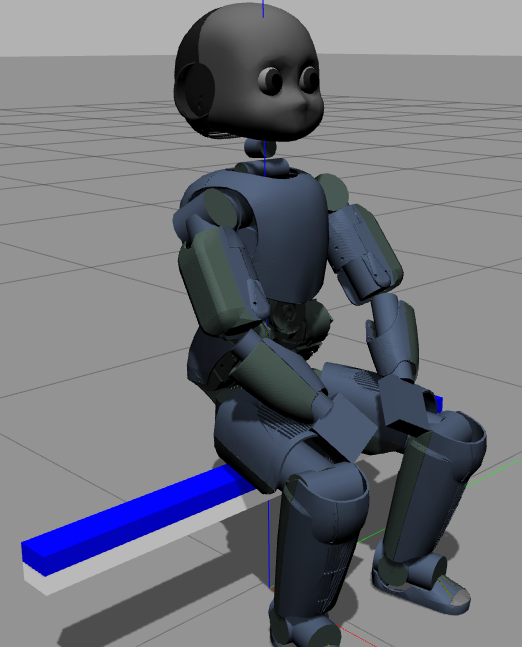
\includegraphics[scale=0.4]{icub_optimum}
  \caption{iCub in optimum sitting configuration.}
  \label{icub_optimum}
\end{figure}
%% %
%% \begin{figure}
%%   \centering
%%   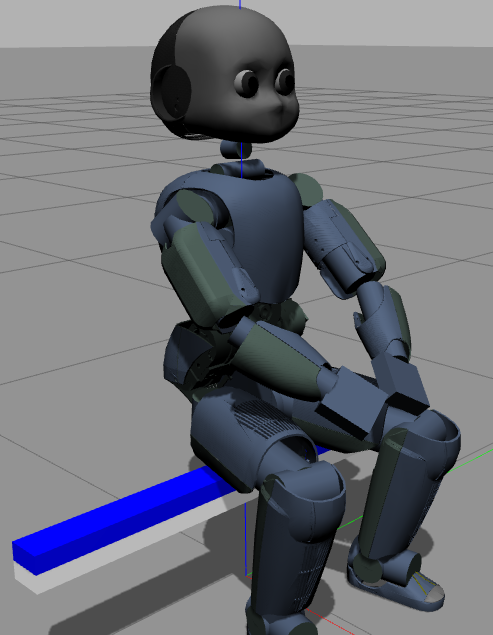
\includegraphics[scale=0.4]{icub_suboptimum}
%%   \caption{iCub in near-optimum sitting configuration.}
%%   \label{icub_suboptimum}
%% \end{figure}
%% %

\emph{Contribution:} Real-time human inverse dynamics computation and visualisation.

\emph{Abstract:} The understanding of the human dynamics and the way in which its contribute can 
be applied to enhance a physical human-robot interaction (pHRI) are two of the 
most promising challenges for the scientific community due mainly to their 
enormous and to-be-developed potential in industrial scenarios, ergonomics 
context, as well as in assistive and rehabilitation fields. 
Classical robots are built to act \emph{for} humans, but in order to adapt 
their functionality to the current technological progress, the new generation 
of robots will have to collaborate \emph{with} humans.  This implies that the 
robots will be endowed with the capability to control physical collaboration 
through intentional interaction with humans.
To achieve this condition, robots have to know mandatorily the dynamics 
(contact forces, internal forces, joint torques) of the human agent who 
they are interacting with.  However the current state of the robot knowledge 
in observing human whole-body dynamics  yields to non-proficient and unadaptive 
interactions.


\emph{4yr Achievements}:
During year four,  IIT investigated a physical-human a pHRI by starting to retrieve the real-time human inverse dynamics estimation during a pHRI (Achievement A1) and the visualisation of the interaction scenario (Achievement A2).

\begin{itemize}
\item[A1] Real-time human inverse dynamics estimation

The core of the analysis consists in the real-time estimation of a dynamic variable $\bm d$ that contains all the information of the kinematics and dynamics of each link (and the related coupled joint) in the human model. 
IIT investigated also the advantage in using this estimation algorithm  by adding progressively  the different sensors data at each computation and the result was that the variance associated to the estimated dynamic variables consequently decreases, making each time the estimation more reliable.

\begin{figure}
  \centering
    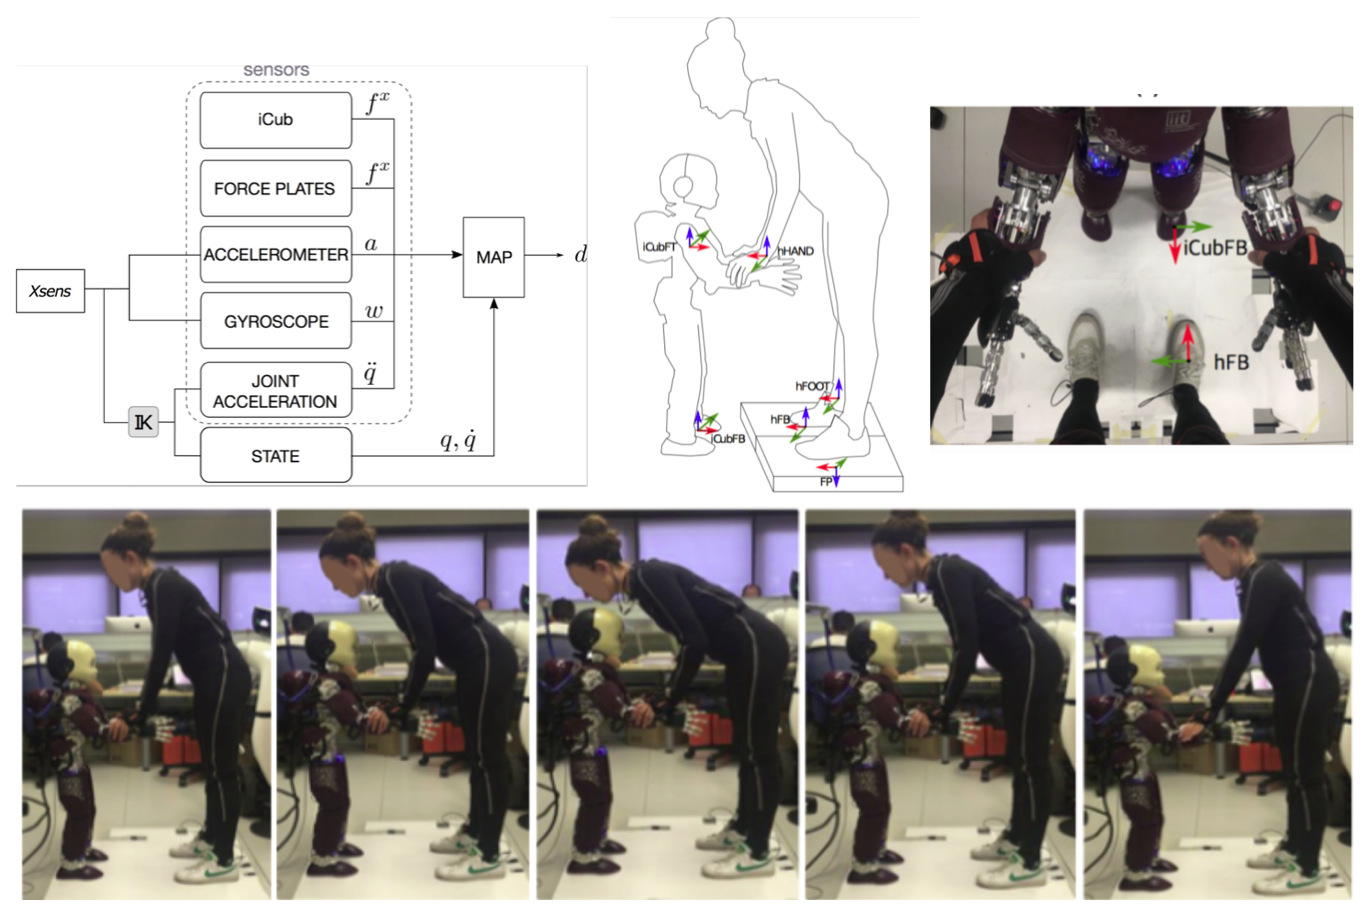
\includegraphics[width=1\columnwidth]{images/full_A1}
  \caption{From left to right: \emph{i)} Overview of the estimation algorithm. \emph{ii)} Sketch of a pHRI experiment where a subject graps and pushes down the robot. \emph{iii)} Top view of the experiment position layout. \emph{iiii)} Sequence of the experimental pHRI.}
 \label{fig:schemeAlgorithm1}
\end{figure}

\begin{figure}
  \centering
    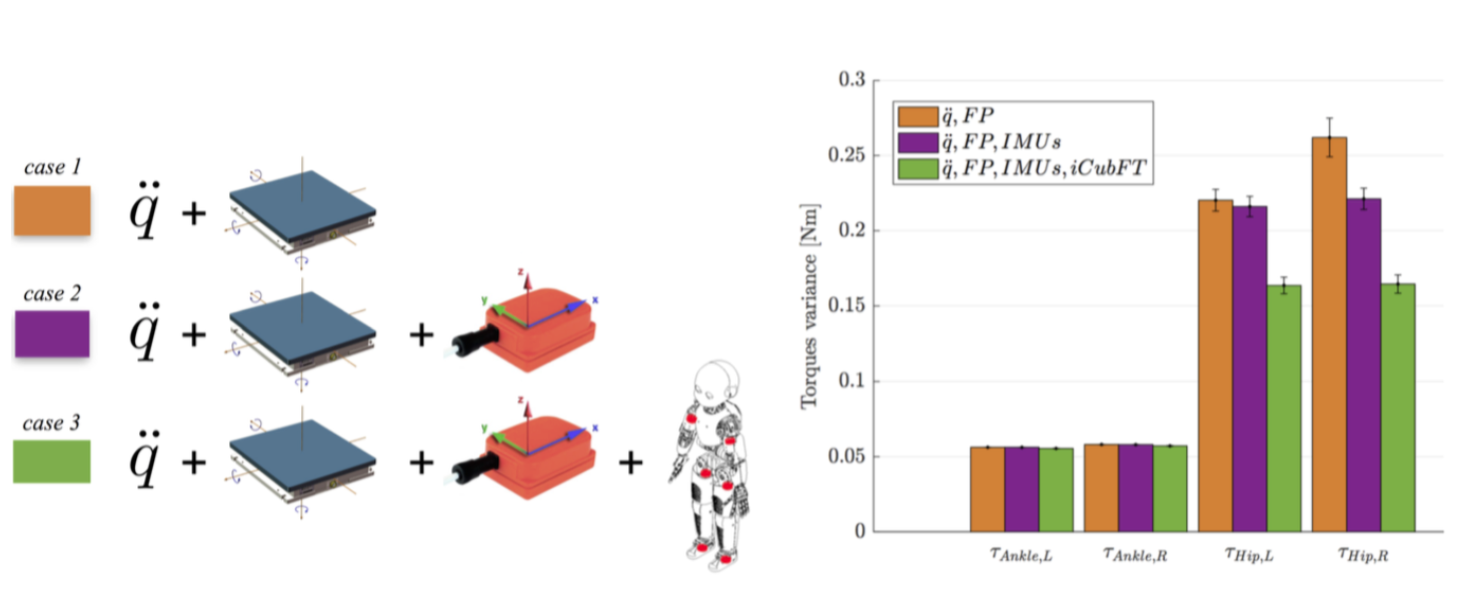
\includegraphics[width=1\columnwidth]{images/sensorFusion_results}
  \caption{From left to right:  \emph{i)} DEscription of three cases for progressive addition of sensors. \emph{ii)} Mean variance of the torque at the left and right ankle in the three sensor cases. }
 \label{fig:schemeAlgorithm2}
\end{figure}


\item[A2] ROS-based visualizer

IIT developed a software component to provide to Rviz (ROS-based visualizer) information about kinematics and dynamics of human subjects while physically interacting with robots.

\begin{figure}
  \centering
    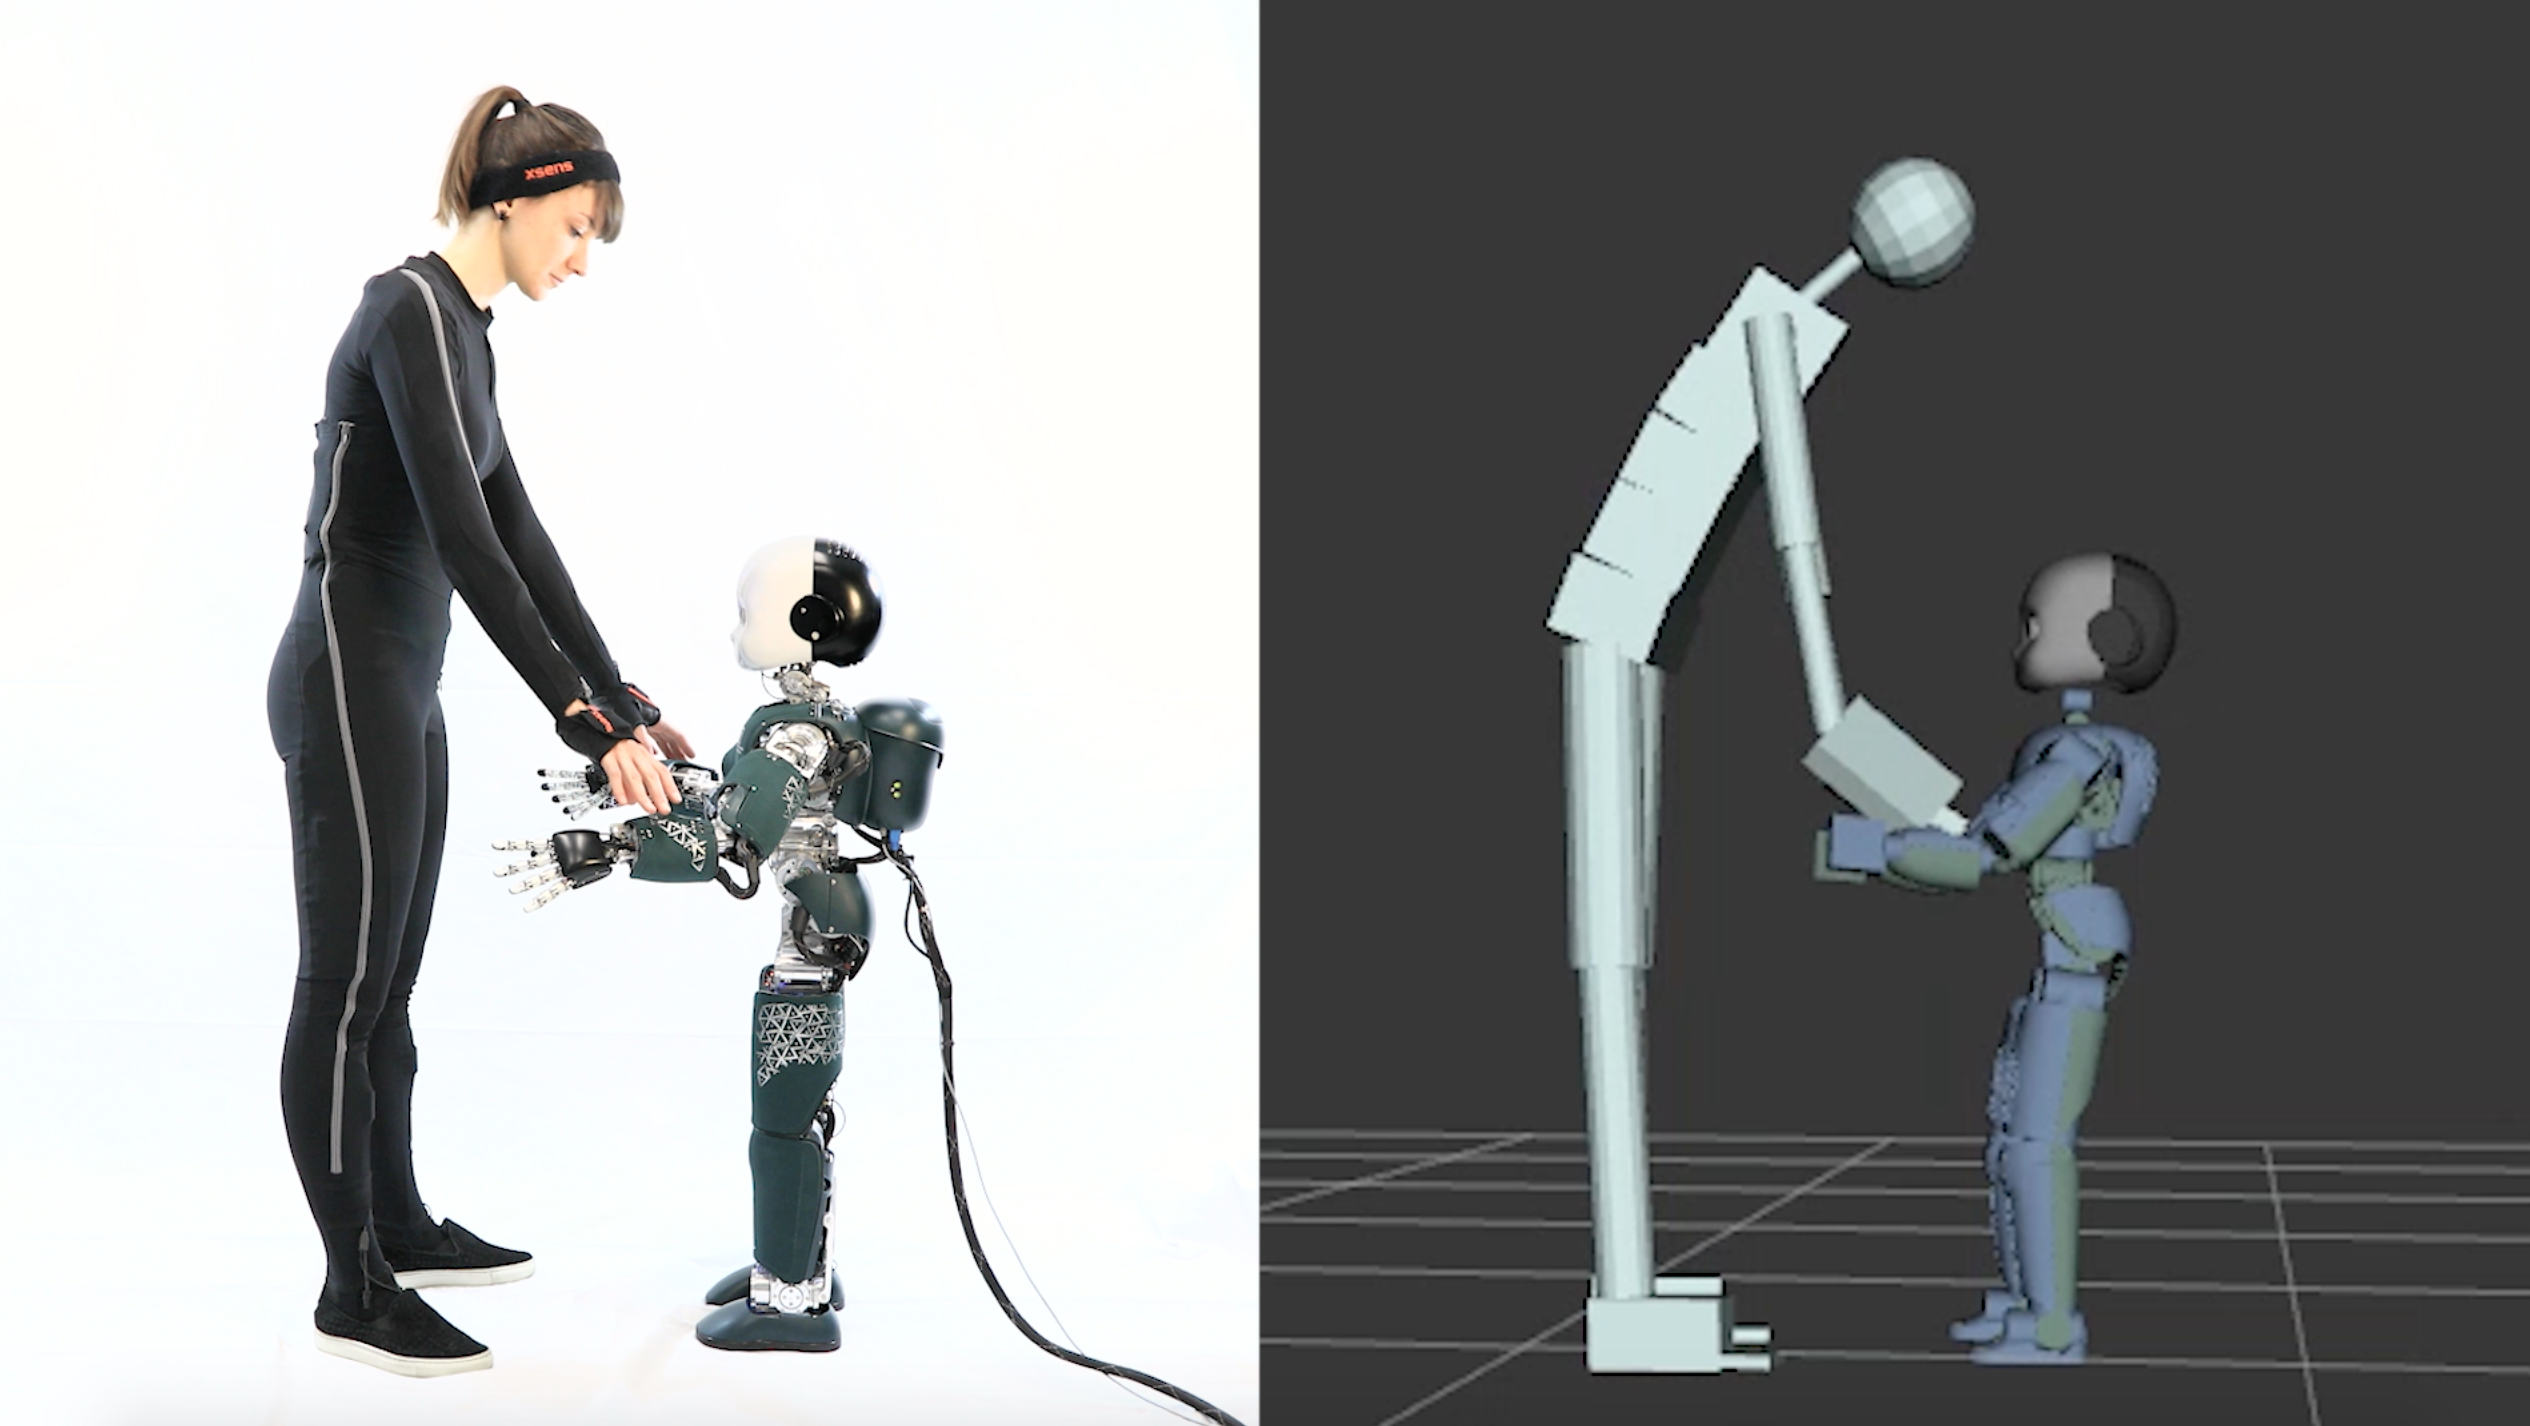
\includegraphics[width=0.8\columnwidth]{images/Rviz_pHRI}
  \caption{Visualizer of pHRI scenario: real interaction (on the left side), viasualization on Rviz for both human and robot models.  }
 \label{fig:schemeAlgorithm3}
\end{figure}

\end{itemize}

%\begin{itemize}
%\item[-] \emph{\color{red}[A summary of progress towards objectives and details for each task;]}
%\item[-] \emph{\color{red}[Highlight clearly significant results;]}
%\item[-] \emph{\color{red}[If applicable, explain the reasons for deviations from Annex I and their impact on other tasks as well as on available resources and planning;]}
%\item[-] \emph{\color{red}[If applicable, explain the reasons for failing to achieve critical objectives and/or not being on schedule and explain the impact on other tasks as well as on available resources and planning (the explanations should be consistent with the declaration by the project coordinator) ;]}
%\item[-] \emph{\color{red}[a statement on the use of resources, in particular highlighting and explaining deviations between actual and planned  person-months per work package and per beneficiary in Annex 1 (Description of Work);]}
%\item[-] \emph{\color{red}[If applicable, propose corrective actions.]}
%\end{itemize}
